% Pôster de TCC - MAC0500 (IME-USP)
% Baseado no template CCSL-IME/USP (Nelson Lago)

%%%%%%%%%%%%%%%%%%%%%%%%%%%%%%%%%%%%%%%%%%%%%%%%%%%%%%%%%%%%%%%%%%%%%%%%%%%%%%%%
%%%%%%%%%%%%%%%%%%%%%%%%%%%%%%%%% PREÂMBULO %%%%%%%%%%%%%%%%%%%%%%%%%%%%%%%%%%%%
%%%%%%%%%%%%%%%%%%%%%%%%%%%%%%%%%%%%%%%%%%%%%%%%%%%%%%%%%%%%%%%%%%%%%%%%%%%%%%%%

\documentclass[a1paper,english,brazilian]{article}

\usepackage{imegoodies}
\usepackage[poster,hidelinks]{imelooks}

% Ponto de equilíbrio entre 21pt (folgado) e 23pt (estourado) para folha A1
\tcbposterset{fontsize = 22pt}

\graphicspath{{figuras/},{fig/},{logos/},{img/},{images/},{imagens/}}

\babeltags{br = brazilian, en = english}

%%%%%%%%%%%%%%%%%%%%%%%%%%%%%%%%%%%%%%%%%%%%%%%%%%%%%%%%%%%%%%%%%%%%%%%%%%%%%%%%
%%%%%%%%%%%%%%%%%%%%%%%%%%%%%%% INÍCIO DO POSTER %%%%%%%%%%%%%%%%%%%%%%%%%%%%%%%
%%%%%%%%%%%%%%%%%%%%%%%%%%%%%%%%%%%%%%%%%%%%%%%%%%%%%%%%%%%%%%%%%%%%%%%%%%%%%%%%

\begin{document}

\begin{tcbposter}[
  poster = {
    %showframe, % descomente se quiser visualizar a grade de alinhamento
    rows = 6,
    columns = 12,
    colspacing = 0.9cm,
    rowspacing = 0.7cm,
  },
]

%%%%%%%%%%%%%%%%%%%%%%%%%%%%%%% CABEÇALHO %%%%%%%%%%%%%%%%%%%%%%%%%%%%%%%%%%%%%%
\posterbox[titlebox]{name=titlebox, below=top, column=1, span=12}{
    Um Sistema Baseado em Redes Neurais\\
    para Detecção de Intrusão em Tráfego DNS\\[0.25cm]
    {\Large Giovanna Luisa Hirata dos Anjos \quad$\cdot$\quad Orientador: Prof. Dr. Daniel Macêdo Batista}\\[0.12cm]
    {\normalsize Bacharelado em Ciência da Computação (MAC0500) --- IME-USP --- 2026}
}

%%%%%%%%%%%%%%%%%%%%%%%%%%%%%%% RODAPÉ %%%%%%%%%%%%%%%%%%%%%%%%%%%%%%%%%%%%%%%%%
\posterbox[footerbox]{name=footerbox, above=bottom, column=1, span=12}{
    \normalsize
    \textbf{Site:} \href{https://www.linux.ime.usp.br/~gihirata/mac0500/}{\texttt{linux.ime.usp.br/\textasciitilde{}gihirata/mac0500}}\par
    \vspace{2pt}
    \textbf{Código (GPLv3):} \href{https://github.com/giovannahirata/IDS-DNS}{\texttt{github.com/giovannahirata/IDS-DNS}}\par
    \vspace{4pt}
    \footnotesize
    \texttt{giovannaluisahirata@usp.br} \quad|\quad \texttt{batista@ime.usp.br}
    \quad---\quad
    \textcolor{imesoftblue!30!white}{DCC -- IME/USP}\relax
    \footimage{%
      \mbox{%
        \raisebox{-0.5\height}{\includegraphics[height=2.4cm]{logo-smartness}}%
        \hspace{0.6cm}%
        \raisebox{-0.5\height}{
\includegraphics[height=1.7cm]{fapesp-logo}}%
        \hspace{0.6cm}%
        \raisebox{-0.5\height}{\includegraphics[height=2.7cm]{ime-logo}}%
        \hspace{0.6cm}%
        \raisebox{-0.5\height}{\includegraphics[height=1.9cm]{usp-logo}}%
      }%
    }
}

%%%%%%%%%%%%%%%%%%%%%%%% LINHA 1: CONTEXTO + METODOLOGIA %%%%%%%%%%%%%%%%%%%%%%%
\posterbox[adjusted title = {1. Contexto, Motivação e Objetivos},
           equal height group = linha1,
           valign = center]
          {name=intro, below=titlebox, column=1, span=7}{

    \begin{minipage}[c]{0.55\textwidth}
      \begin{itemize}\setlength{\itemsep}{4pt}
        \item \textbf{Problema:} ataques de \texten{phishing}, \texten{malware} e \texten{spam} dependem de domínios maliciosos criados a todo segundo. Listas de bloqueio são reativas e a derrubada burocrática é lenta.
        \item \textbf{Caso real (USP, jun/2025):} o clone \texttt{uspdigital.com.br} permaneceu no ar por mais de 12 dias mesmo após notificação da STI.
        \item \textbf{Por que DNS?} Protocolo que traduz nomes de domínio em endereços IP antes de qualquer acesso na Internet e costuma trafegar sem criptografia, permitindo bloqueio proativo.
        \item \textbf{Objetivos:} desenvolver um IDS proativo baseado em redes neurais, auditar atributos via SHAP, especializar para domínios \texttt{.br} e validar socialmente no Eixo de Extensão.
      \end{itemize}
    \end{minipage}\hfill
    \begin{minipage}[c]{0.42\textwidth}
      \centering
      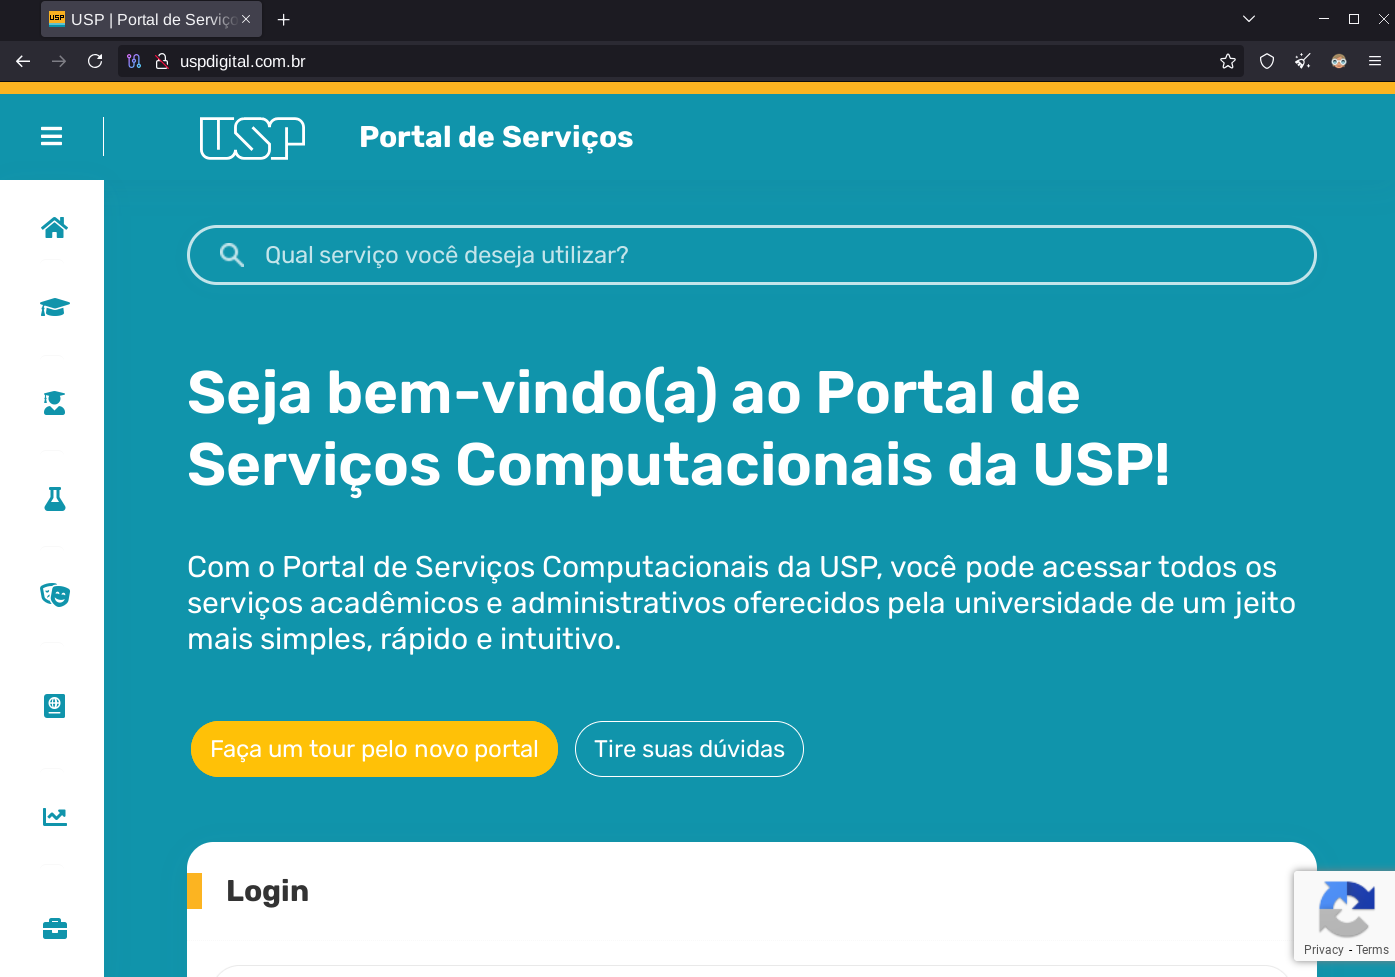
\includegraphics[width=\linewidth,height=11.5cm,keepaspectratio]{site-falso-usp}\par
      \vspace{5pt}
      {\footnotesize Clone do Portal de Serviços da USP hospedado em \texttt{uspdigital.com.br}.}
    \end{minipage}
}

\posterbox[adjusted title = {2. Dataset e Arquitetura Proposta},
           equal height group = linha1,
           valign = center]
          {name=metodo, below=titlebox, column=8, span=5}{

    \begin{minipage}[c]{0.55\textwidth}
      \begin{itemize}\setlength{\itemsep}{4pt}
        \item \textbf{Dataset \texttt{BCCC-CIC-Bell-DNS-2024}:} 3.595.920 fluxos DNS e 122 features (rede/transporte, aplicação/TTL e lexicais).
        \item \textbf{Distribuição real:} 95,68\% benigno, 2,27\% \texten{malware}, 1,21\% \texten{phishing} e 0,84\% \texten{spam}.
        \item \textbf{Modelos avaliados:} SVM, KNN e MLP (TensorFlow) com 3 camadas densas ($128 \rightarrow 64 \rightarrow 32$, ReLU), \texten{Dropout} 30\%, \texten{EarlyStopping} e saídas \texten{sigmoid} (binária) e \texten{softmax} (multiclasse).
      \end{itemize}
    \end{minipage}\hfill
    \begin{minipage}[c]{0.42\textwidth}
      \centering
      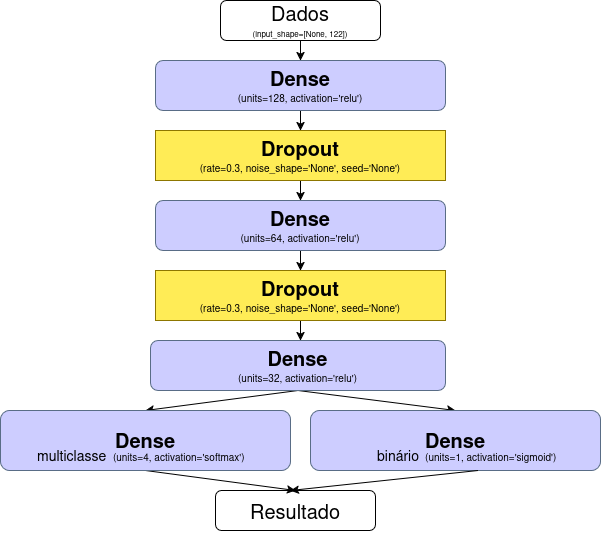
\includegraphics[width=\linewidth,height=13.0cm,keepaspectratio]{mlp-diagram.drawio.png}\par
      \vspace{3pt}
      {\footnotesize Arquitetura da rede MLP.}
    \end{minipage}
}

%%%%%%%%%%%%%%%%% LINHA 2: EXPLICABILIDADE + RESULTADOS/.BR %%%%%%%%%%%%%%%%%%%%
\posterbox[adjusted title = {3. Explicabilidade (SHAP) e Descoberta de Viés},
           equal height group = linha2,
           valign = center]
          {name=shapbox, below=intro, column=1, span=6}{

    \begin{itemize}\setlength{\itemsep}{6pt}
      \item \textbf{Viés oculto encontrado:} a auditoria via SHAP revelou que a porta de origem (\texttt{src\_port}) dominava as decisões por um artefato da coleta em laboratório, que associou portas fixas às classes (benigno: 58075/53; \texten{malware}/\texten{phishing}: 46177).
      \item \textbf{Impacto da remoção da \textit{feature} \texttt{src\_port} (dados desbalanceados):} SVM binário caiu de F1 0,8933 para \textcolor{imered}{\textbf{0,2044}} e KNN de 0,9758 para 0,6130. A \textbf{MLP multiclasse} manteve estabilidade (\textbf{F1 = 0,9968}), aprendendo padrões comportamentais reais.
    \end{itemize}

    \vspace{1.7cm}

    \noindent
    \begin{minipage}[t]{0.48\textwidth}
      \centering
      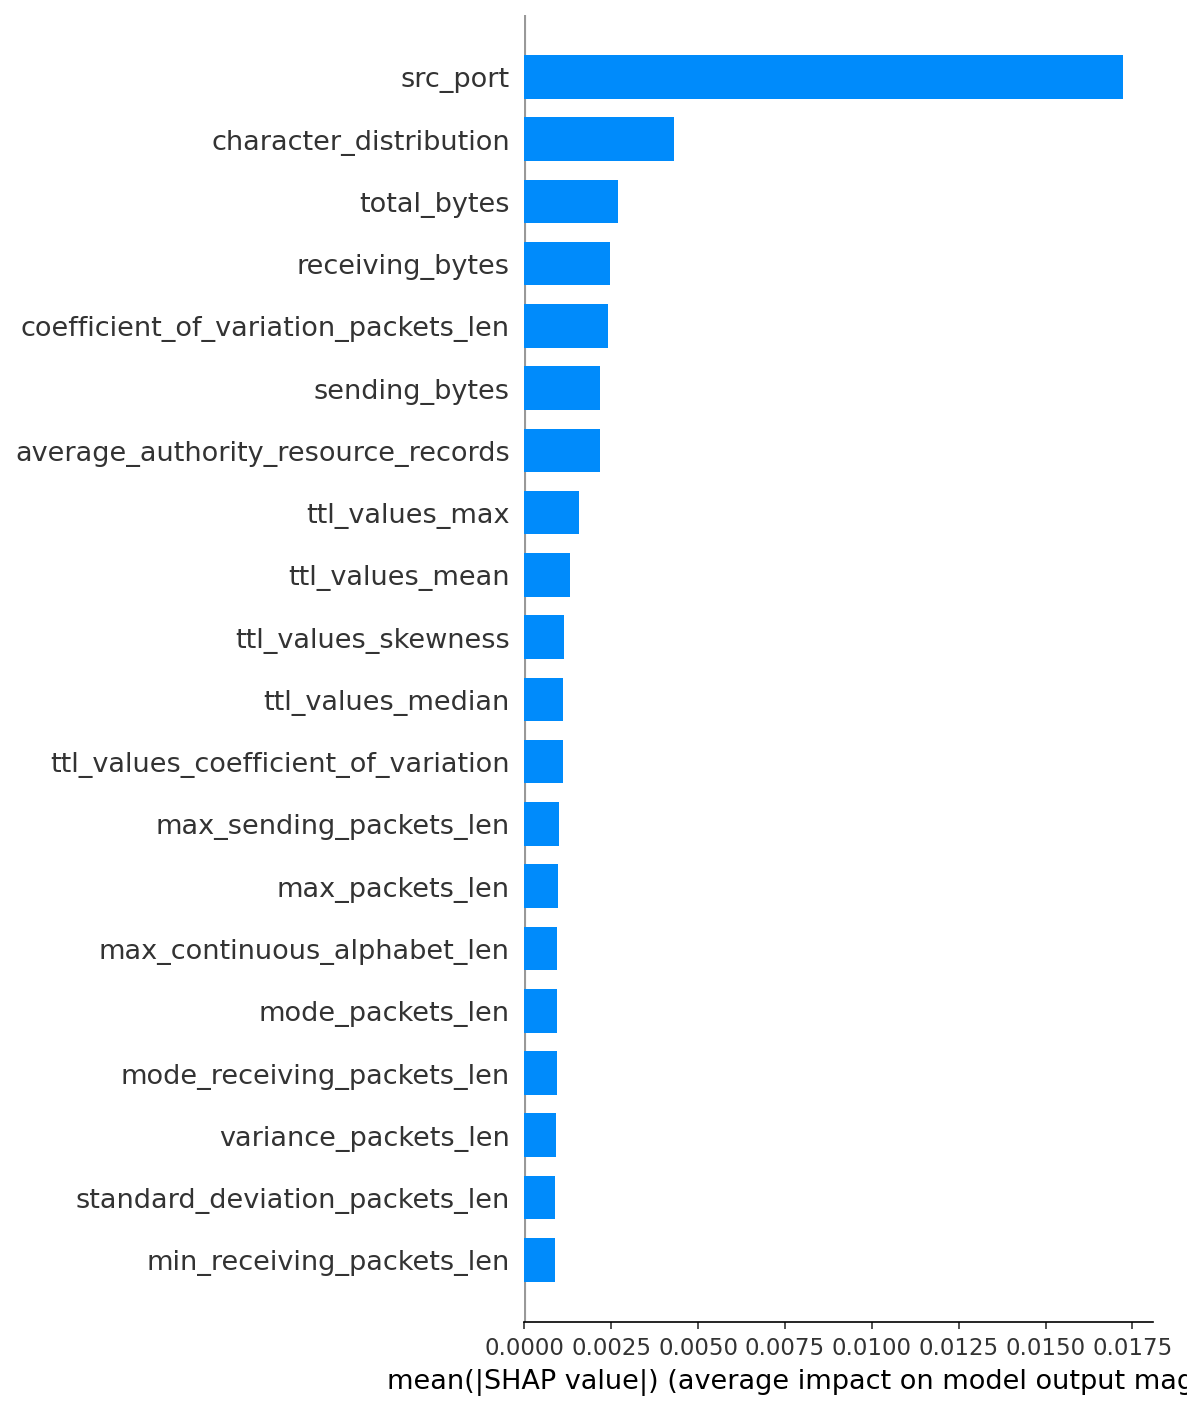
\includegraphics[width=\linewidth,height=12.0cm,keepaspectratio]{shap_bar_plot_antes}\par
      \vspace{4pt}
      {\footnotesize \textit{Antes:} decisão dominada por \texttt{src\_port}.}
    \end{minipage}\hfill
    \begin{minipage}[t]{0.48\textwidth}
      \centering
      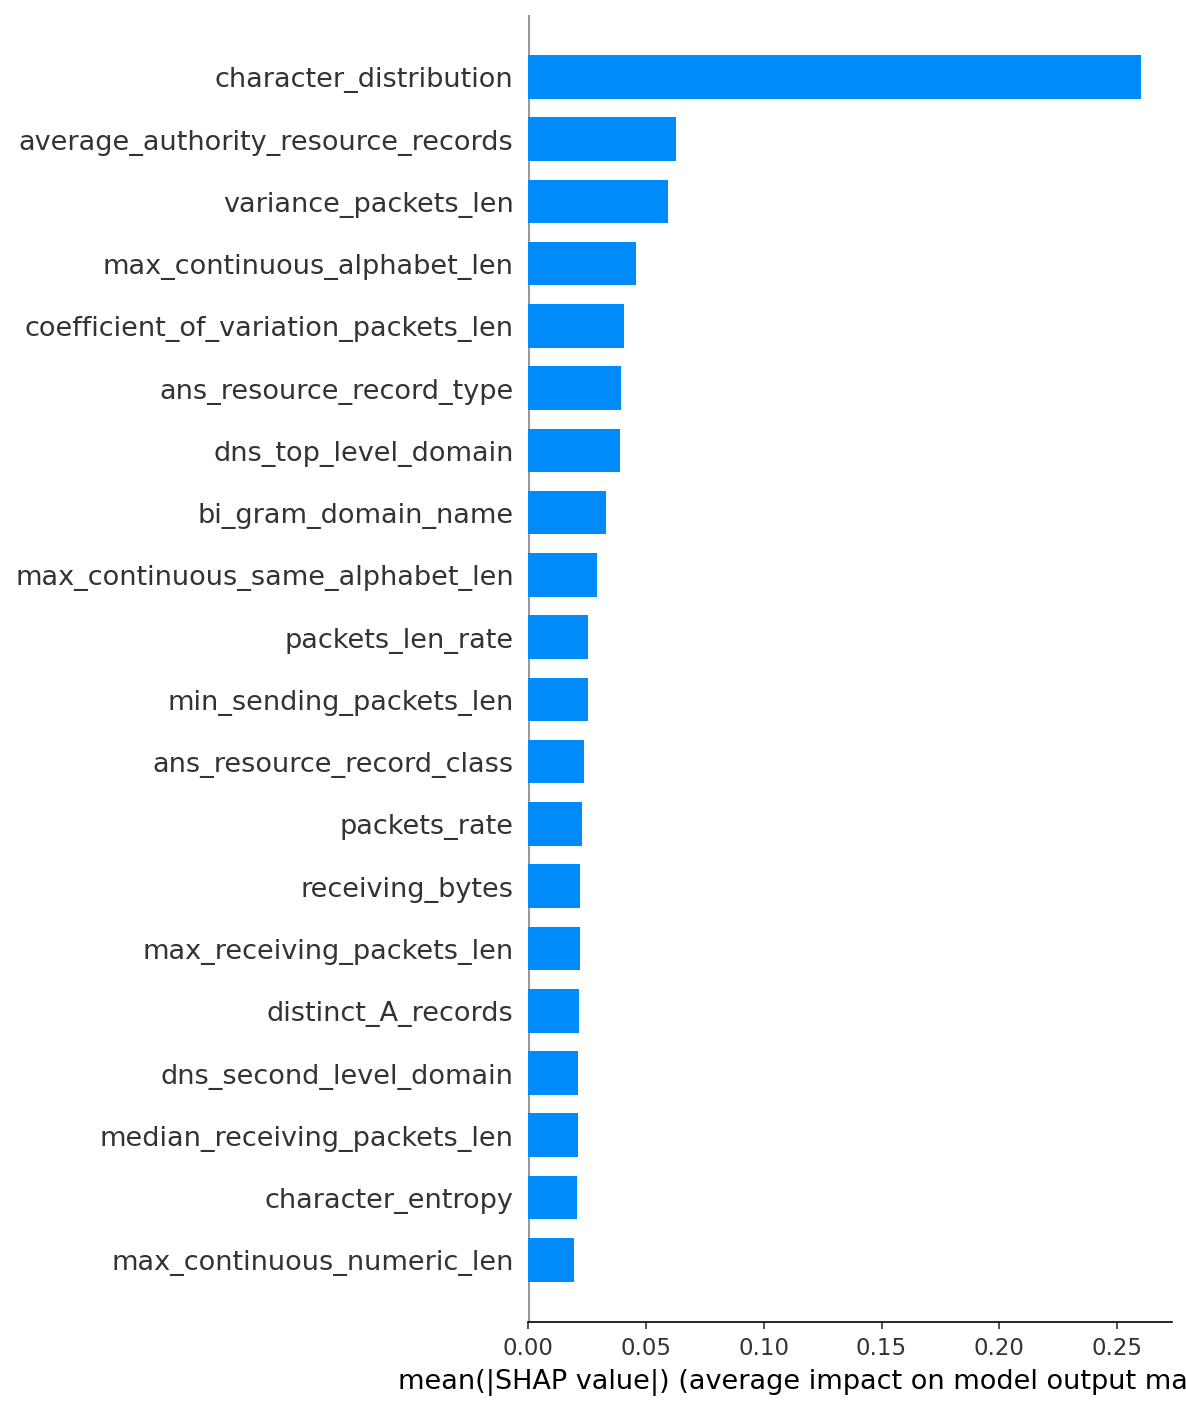
\includegraphics[width=\linewidth,height=12.0cm,keepaspectratio]{shap_bar_plot-depois_sem_src_port_balanceado}\par
      \vspace{4pt}
      {\footnotesize \textit{Depois:} features comportamentais e lexicais.}
    \end{minipage}
}

\posterbox[adjusted title = {4. Desempenho Balanceado e Especialização (.br)},
           equal height group = linha2,
           valign = center]
          {name=resbr, below=metodo, column=7, span=6}{

    \begin{minipage}[c]{0.55\textwidth}
      \textbf{1) Balanceamento de classes (sem \texttt{src\_port}):}\\
      {\footnotesize Como o dataset original tem 95,7\% de tráfego benigno, balanceou-se as classes (média de 10 execuções, divisão 70\% treino / 30\% teste) para evitar falsos negativos em ataques menos frequentes:}\\[5pt]
      \resizebox{\linewidth}{!}{%
        \renewcommand{\arraystretch}{1.2}%
        \begin{tabular}{lccc}
          \toprule
          Classe (MLP Multiclasse) & Precisão & Recall & F1-Score \\
          \midrule
          Benigno  & 0,942 $\pm$ 0,007 & 0,965 $\pm$ 0,005 & \textbf{0,953 $\pm$ 0,003} \\
          Malware  & 0,820 $\pm$ 0,014 & 0,836 $\pm$ 0,017 & \textbf{0,828 $\pm$ 0,007} \\
          Phishing & 0,864 $\pm$ 0,023 & 0,796 $\pm$ 0,023 & \textbf{0,828 $\pm$ 0,017} \\
          Spam     & 0,840 $\pm$ 0,021 & 0,786 $\pm$ 0,024 & \textbf{0,812 $\pm$ 0,017} \\
          \bottomrule
        \end{tabular}%
      }\\[10pt]
      \textbf{2) Modelo especializado em \texttt{.br} vs. Internacional:}\\
      {\footnotesize Filtro apenas dos \textbf{27.711 fluxos \texttt{.br}} e comparação com a MLP treinada na base internacional completa:}\\[5pt]
      \resizebox{\linewidth}{!}{%
        \renewcommand{\arraystretch}{1.2}%
        \begin{tabular}{lccc}
          \toprule
          Classificação & F1 (\texttt{.br}) & F1 (Internacional) & AUC-ROC (\texttt{.br}) \\
          \midrule
          Binária     & 0,8739 & 0,9093 & 0,9877 \\
          Multiclasse & \textbf{0,9173} & 0,9282 & \textbf{0,9866} \\
          \bottomrule
        \end{tabular}%
      }\\[6pt]
      {\footnotesize \textbf{Conclusão:} mesmo treinado com menos de 1\% dos dados, o modelo \texttt{.br} ficou próximo ao internacional (diferença $<$ 3 pontos percentuais na maioria das métricas) e manteve inferência ultrarrápida ($\approx$ 0,017 ms/amostra), comprovando a viabilidade de especialização nacional.}
    \end{minipage}\hfill
    \begin{minipage}[c]{0.42\textwidth}
      \centering
      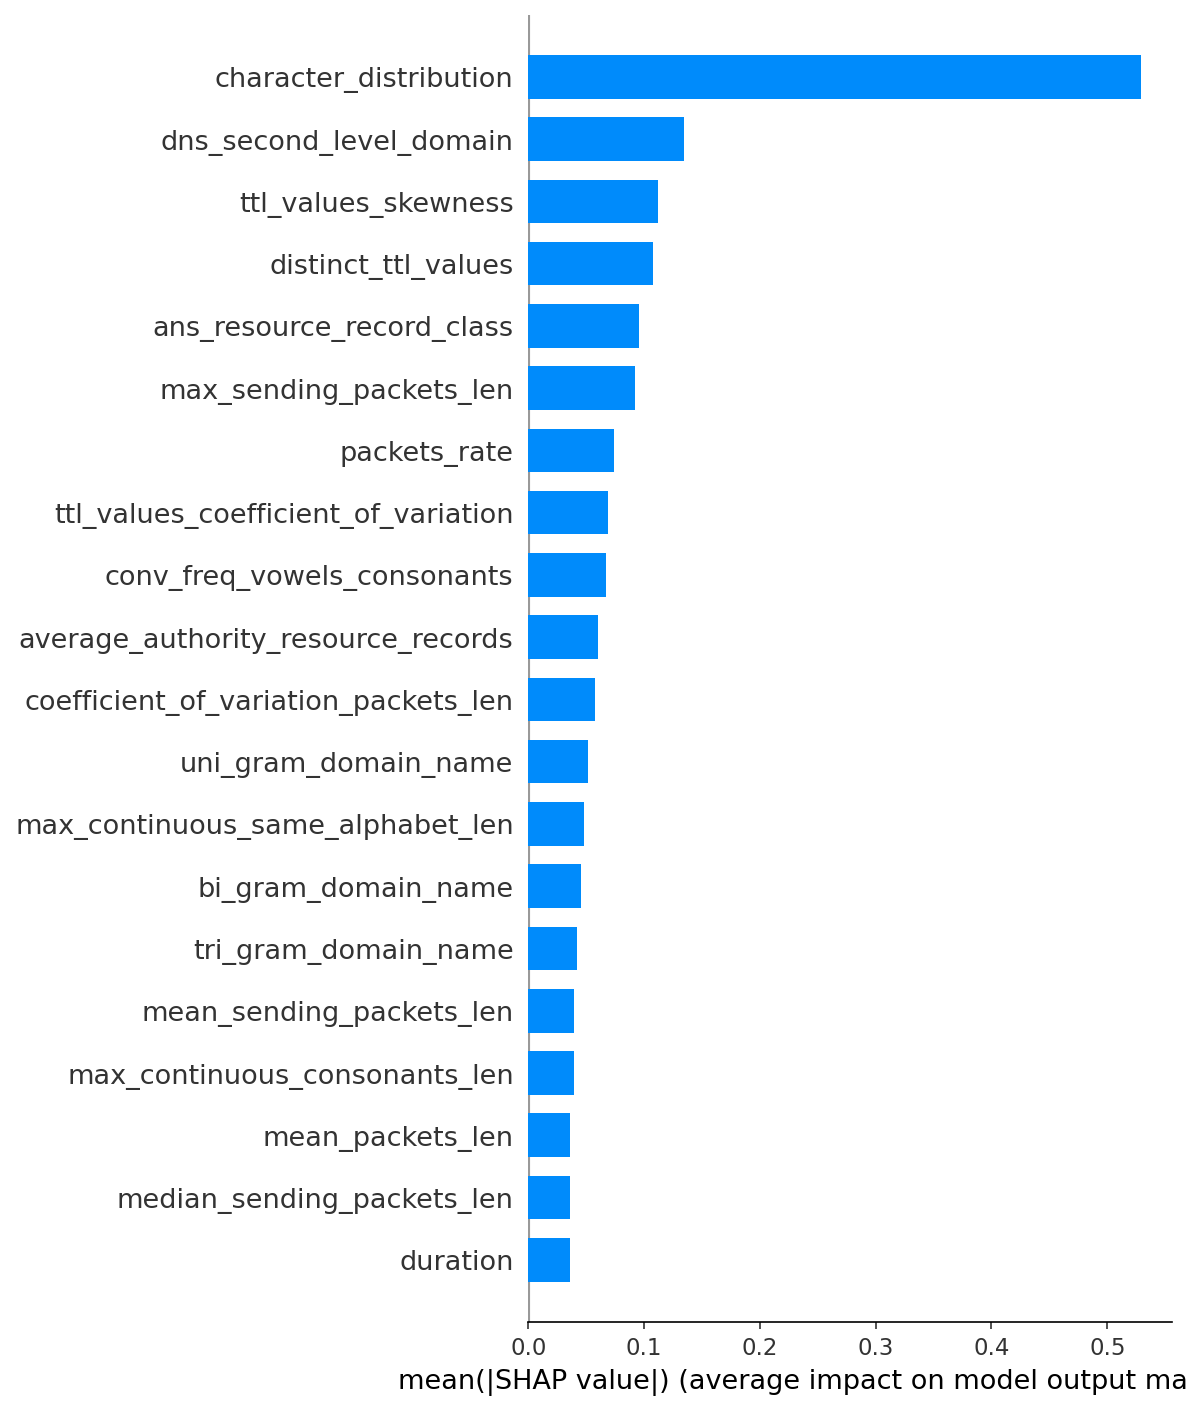
\includegraphics[width=\linewidth,height=14.0cm,keepaspectratio]{shap_bar_plot_br}\par
      \vspace{4pt}
      {\footnotesize \textbf{Atributos mais decisivos em \texttt{.br} (SHAP):} distribuição de caracteres (\texttt{character\_distribution}), nome de segundo nível do domínio (\texttt{dns\_second\_level\_domain}) e estatísticas de tempo de vida em cache (TTL).}
    \end{minipage}
}

%%%%%%%%%%%%%%%%%% LINHA 3: EXTENSÃO + PIPELINE/CONCLUSÕES %%%%%%%%%%%%%%%%%%%%%
\posterbox[adjusted title = {5. Eixo de Extensão: Validação Social (Pessoas vs. IA)}]
          {name=extensao, between=shapbox and footerbox, column=1, span=7}{

    \textbf{Protocolo:} formulário cego com \textbf{200 domínios \texttt{.br}} (100 legítimos e 100 maliciosos), avaliados por \textbf{12 pessoas sem formação em TI}, \textbf{1 especialista em segurança} e pelos modelos MLP via captura real de tráfego DNS.\par
    \vspace{10pt}

    \noindent
    {\setlength{\fboxsep}{5pt}%
    \colorbox{imesoftblue!15!white}{%
      \begin{minipage}[c]{0.295\linewidth}
        \centering\vspace{4pt}
        {\large\textbf{95\% vs. 43\%}}\\[2pt]
        {\footnotesize Acurácia: MLP vs. Público}
        \vspace{4pt}
      \end{minipage}%
    }\hfill
    \colorbox{imesoftblue!15!white}{%
      \begin{minipage}[c]{0.295\linewidth}
        \centering\vspace{4pt}
        {\large\textbf{2\%--4\% de FN}}\\[2pt]
        {\footnotesize vs. 58\%--67\% nos humanos}
        \vspace{4pt}
      \end{minipage}%
    }\hfill
    \colorbox{imesoftblue!15!white}{%
      \begin{minipage}[c]{0.295\linewidth}
        \centering\vspace{4pt}
        {\large\textbf{$>$ 50$\times$ mais rápido}}\\[2pt]
        {\footnotesize $\approx$ 47 ms por domínio}
        \vspace{4pt}
      \end{minipage}%
    }}\par
    \vspace{12pt}

    \centering
    \resizebox{\linewidth}{!}{%
      \renewcommand{\arraystretch}{1.28}%
      \begin{tabular}{lcccc}
        \toprule
        Avaliador / Modelo & Acurácia & Falso Neg. (FN) & Falso Pos. (FP) & Tempo Total \\
        \midrule
        Especialista em Segurança & 36,50\% & \textcolor{imered}{\textbf{67,00\%}} & 60,00\% & 8 min 24 s \\
        Média do Público Externo  & 43,00\% & \textcolor{imered}{\textbf{57,75\%}} & 56,25\% & 11 min 36 s \\
        \textbf{Modelo MLP Binário}     & \textbf{93,00\%} & \textbf{2,00\%} & 12,00\% & \textbf{9,77 s} \\
        \textbf{Modelo MLP Multiclasse} & \textbf{95,00\%} & \textbf{4,00\%} & \textbf{6,00\%} & \textbf{9,41 s} \\
        \bottomrule
      \end{tabular}%
    }\par
    \vspace{12pt}

    \raggedright
    \textbf{Conclusão sociotécnica:} tanto o público externo quanto o especialista tiveram desempenho inferior ao acaso (50\%) devido ao viés de familiaridade e ao \texten{typosquatting}. Enquanto a MLP binária obteve o menor FN (2\%), a multiclasse reduziu falsos positivos (6\%). Logo, a proteção deve atuar de forma automatizada na rede, sem delegar a detecção visual ao usuário final.
}

\posterbox[adjusted title = {6. Arquiteturas Híbridas e Pipeline em Tempo Real}]
          {name=pipeline, below=resbr, column=8, span=5}{

    \begin{itemize}\setlength{\itemsep}{4pt}
      \item \textbf{Ensemble MLP+CNN+LSTM:} alcançou 99,60\% de acurácia e AUC-ROC de \textbf{0,9875}, mas precisão de 0,46 e F1 de 0,57 na classe maligna (126 malignas vs.\ 35.367 benignas), mostrando que a acurácia geral engana em dados desbalanceados.
      \item \textbf{Pipeline em tempo real:} recebe um domínio, captura o tráfego DNS ativo, extrai features comportamentais/lexicais via \texttt{ALFlowLyzer} (sem \texttt{src\_port}) e classifica com a MLP.
    \end{itemize}
}

\posterbox[adjusted title = {7. Conclusões, Reconhecimento e Apoio},
           colframe = imeyellow]
          {between=pipeline and footerbox, column=8, span=5}{

    \begin{itemize}\setlength{\itemsep}{5pt}
      \item \textbf{Resultados centrais:} IDS proativo baseado em MLP com F1 médio de \textbf{0,95} (benigno) e \textbf{0,82} (malicioso), validado via auditoria SHAP e público externo.
      \item \textbf{Publicação:} artigo nos Anais Estendidos do \textbf{XLIV SBRC 2026}.
      \item \textbf{Trabalhos futuros:} dataset nativo \texttt{.br}, bloqueio automático em DNS/\texten{firewall} (ex.: eBPF/XDP), NAS e testes em produção.
      \item \textbf{Apoio:} FAPESP (proc. 25/22251-2) e CPE SMARTNESS (FAPESP 21/00199-8).
    \end{itemize}
}

\end{tcbposter}

\end{document}